%%%%%%%%%%%%%%% Seleccion del tipo de documento y formato de página%%%%%%%%%%%%%

\documentclass[oneside,% formato de páginas de un solo lado
               openany,% los capítulos pueden empezar en cualquier página
               letterpaper,% tamaño de papel ocho y medio por onze
               12pt]% tamaño de letra normal de 12pt 
               {book} % clase libro
\usepackage{geometry} % permite dar opciones de configuración de página
\geometry{top=1in,% tamaño del margen superior
          bottom=1in,% tamaño del margen inferior
          left=1.5in,% tamaño del margen izquierdo
          right=1in,% tamaño del margen derecho
          showframe=false % muestra los marcos de las cajas
         }% -- margin,marginparwidth, landscape,a4paper
          
%%%%%%%%%%%%%%%%%% Configuración de los encabezados de capítulos, secciones y demás%%%%%%%%%%%%%%%%%%%%%
%\usepackage{titletoc} % permite modificar el estilo del índice general
\usepackage[tiny]{titlesec} % permite modificar los encabezados de las distintas partes del documento
\usepackage{color}% permite añadir colores al documento
\definecolor{gray75}{gray}{0.75} %define el comando para un color
\newcommand{\hspdiez}{\hspace{10pt}} % crea un nuevo comando para dejar un espacio horizontal de 10 pt
\titleformat{\chapter}[hang]{\centering\Large\bfseries}{\thechapter.\hspdiez}{0pt}{\Large\bfseries}
%\titleformat{\section}{\normalfont\bfseries}{\thesection.}{0.5em}{\normalfont\bfseries}
\titlespacing{\chapter}{0pt}{-5ex}{5ex}
%%%%%%%%%%%%%%%%%%%%%%%%%Configurar el encabezado y pie de página%%%%%%%%%%%%%%%%%%

\usepackage{fancyhdr}
\fancyhf{}
\rhead{\thepage}
\renewcommand{\headrulewidth}{0pt}
\fancypagestyle{plain}{%
	\fancyhf{}
	\rhead{\thepage}
	\renewcommand{\headrulewidth}{0pt}}
\pagestyle{fancy}
\setlength{\headheight}{15pt}
%%%%%%%%%%%%%%%%%%%%%%%%Configuración general%%%%%%%%%%%%%%%%%%%%%%%%%%%%%%%%%%
\usepackage[utf8]{inputenc} % compatibilidad con encoding utf8, de manera que se pueden codificar directamente ciertos caracteres especiales en latex como los acentos
\usepackage[T1]{fontenc} % paquete relacionado con el encoding de las letras en el documento
\usepackage[spanish,es-tabla,english]{babel} %permite la compatibilidad con diferentes idiomas
\usepackage{mathptmx}  % Letra Times New Roman; otros tipos de letra (e.g. lmodern)
\usepackage{microtype} % mejor tipografía para pdflatex
\usepackage{csquotes} % mejores comillas
\usepackage[shortlabels]{enumitem} % añade mejor control para la configuración de listas
\usepackage{setspace} % permite configurar los espacios de interlineado

\usepackage{lipsum} % permite introducir texto Lorem Ipsum para probar el formato de la página
\usepackage{indentfirst} % Crea una sangría en el primer párrafo de cada capítulo, si se desea el estilo predeterminado comentar esta línea
\settowidth{\parindent}{~~~~~}% introduce una sangría de 5 espacios
%\setlength\parindent{5ex} % argumento para modificar el tamaño de las sangrías en el texto. Comentar esta línea para obtener el valor predeterminado
\usepackage{siunitx} % configura unidades de medidas en ciencia
\usepackage{pdflscape} % cambia la orientación de la página deseada
\usepackage{etoc} % permite separar el índice general en partes (e.g. índice de anexos)
\usepackage{verbatim} % permite hacer comentarios de varias líneas
%%%%%%%%%%%%%Configuración de figuras y tablas%%%%%%%%%
\usepackage{tabu} % crea un ambiente nuevo para tablas con más funciones
\usepackage{booktabs} % mejores reglas horizontales para tablas
\usepackage{array} % permite más control del tamaño de celdas en una tabla
\usepackage{longtable} % permite tablas que se extiendan más de una página
\usepackage{dcolumn}
\newcolumntype{d}[1]{D{.}{\cdot}{#1} }
\newcommand{\cabeza}[1]{\textbf{#1}}
%\setlength{\extrarowheight}{5pt} % produce espacio extra entre las filas
%\setlength{\abovetopsep}{1ex} % set space left above toprule
\setlength{\heavyrulewidth}{1.5pt} % width of both top and bottom rule
\usepackage[font=small,labelfont=bf,margin=1cm]{caption} % mejora el título de figuras y tablas
\usepackage{chngcntr} % permite la numeración continua de las tablas y figuras
\counterwithout{figure}{chapter} % numeración de las figuras no se reinicia con cada capítulo
\counterwithout{table}{chapter} % numeración de las tablas no se reinicia con cada capítulo
\usepackage{graphicx} % permite añadir y manejar imágenes en el documento
\graphicspath{ {./imagenes/} } % localidad del archivo de imagenes
\usepackage{subcaption} % permite múltiples figuras
%%%%%%%%%%%%%%%%%%%%% Configuración de la bibliografía %%%%%%%%%%%%%%%%%
%%%%%%%%%Confguración en Biblatex%%%%%%%%%
\usepackage[%
backend=biber,% utiliza biber para procesar el archivo de bibliografía
style=authoryear-icomp,% estilo de citas por autor y año
sorting=nyt,% orden de las citas por nombre, año y título
natbib=true,% permite compatibilidad con los comandos citep{} y citet{} de natbib
uniquename=init,% crea la lista de nombres únicos incluyendo las iniciales
giveninits,% usa las iniciales de los autores en la bibliografía
url=false,% no imprime el url en la bibliografía
doi=false,% no imprime el doi en la bibliografía
isbn=false,% no imprime el isbn del libro
hyperref=true,% permite links en la cita
maxbibnames=99,% número de autores impresos en la bibliografía
maxcitenames=2]% permite un máximo de dos autores en la citas
{biblatex} % paquete que permite la configuración de las citas bibliográficas
%\DeclareNameAlias{sortname}{last-first}
%%%\DeclareFieldFormat[article]{title}{#1}
%%%\DeclareFieldFormat[article]{journaltitle}{#1}
\DeclareFieldFormat[book]{title}{#1}
\DeclareFieldFormat[article]{pages}{#1}
\DeclareFieldFormat[book,incollection,inbook]{pages}{#1 pp}
%\DeclareFieldFormat{editor}{#1}
\DeclareFieldFormat{booktitle}{#1}
\DeclareFieldFormat[article,inbook,incollection,inproceedings,patent,thesis,unpublished]{title}{#1\isdot} % remueve las comillas de los títulos en la bibliografía
\DeclareFieldFormat[article]{journaltitle}{#1} % escribe el nombre de la revista en letra normal y no italizada
\DefineBibliographyStrings{spanish}{%
	andothers={et~al\adddot},% las citas con más de dos autores terminarán en "et. al" y no en "y col." 
	bibliography={Literatura Citada}} % cambia el título de la bibliografía por Literatura Citada
\renewbibmacro{in:}{%
 \ifentrytype{article}{}{\printtext{\bibstring{in}\intitlepunct}}}
%%%%%%%%%%%%%%%%fin biblatex%%%%%%%%%%%
%%%%%%%%%% configuración bibliografía con xpatch%%%%%%
%%Configuración artículo%%%%
\usepackage{xpatch}
\xpatchbibmacro{journal+issuetitle}{%
  \setunit*{\addspace}%
  \iffieldundef{series}}
  {%
  \setunit*{\addcomma\space}%
  \iffieldundef{series}}{}{}

\renewcommand\bibpagespunct{\ifentrytype{article}{\addcolon}{\addcomma}\space}
\renewbibmacro*{volume+number+eid}{%
  \printfield{volume}
  \printfield[parens]{number}%
  \setunit{\addcomma\space}%
  \printfield{eid}}

\xpatchbibmacro{date+extrayear}{%
  \printtext[parens]%
}{%
  \setunit*{\addperiod\space}%
  \printtext%
}{}{}

%%% Configuración capítulo libro
\DeclareNameAlias{editorin}{first-last}
\newbibmacro*{byeditor:in}{%
  \ifnameundef{editor}
    {}
    {\printnames[editorin]{editor}%
     \addcomma\addspace%
     \usebibmacro{editorstrg}}%
     \clearname{editor}%
     \printunit{\addperiod\space}}
     
\xpatchbibdriver{incollection}
  {\usebibmacro{in:}%
   \usebibmacro{maintitle+booktitle}%
   \newunit\newblock
   \usebibmacro{byeditor+others}}
  {\usebibmacro{in:}%
   \usebibmacro{byeditor:in}%
   \setunit{\labelnamepunct}\newblock
   \usebibmacro{maintitle+booktitle}%
   \newunit\newblock
   \usebibmacro{byeditor}}
  {}{}

\addbibresource{referencias.bib} % nombre del archivo con las referencias en formato bib(la)Tex




%%%%%%%%%%Declaración para biblatex 3.4 y biber 2.5%%%%%%%%%%%%%%%%%%%%%%%%%%
%%%	SOLUCIÓN NO FUNCIONA PARA BIBLATEX 3.3 Y NO ES NECESARIO A PARTIR DE LA VERSIÓN 3.5
%\DeclareDelimFormat[cbx@textcite]{nameyeardelim}{\addspace} % se necesita para compensar un bug de la versión 3.4 biblatex donde cita de la manera autor, (año) en lugar de autor (año).

%\DeclareNameAlias{sortname}{last-first}
%%%%%%%%%%%%%%%%%%%%%%%%%%%%%%%%%%%%%%%%%%%%%%%%%%%%%%%%%%%%%%%%%%%%%%%%%%%%%%%%%%%

\usepackage[colorlinks=true, allcolors=black]{hyperref} % permite la creación de links en el texto, es mejor cargar este paquete al final del preámbulo

%%%%%%%%%%%%%%%% Paquetes opcionales, chequear la describción %%%%%%%%%%%%%%%%%%%%%%
%\usepackage{parskip} % maneja la identación de los párrafos, mirar mejor
%\usepackage{url} % mejor compatibilidad con enlaces url en el texto
%\usepackage{todonotes} % add notes of things to add to the manuscript
%\usepackage{verbatim} % permite crear comentarios multilínea
% % handle line spacing


%\includeonly{introduccion} % utilizar para filtrar que capítulos mostrar en el texto
\begin{document}
\frontmatter
\etocdepthtag.toc{general} % configura a partir de donde crear el índice general
\begin{titlepage}
\begin{center}
\setlength{\parindent}{0cm}

\textsc{\Large Universidad Autónoma de Santo Domingo\\
Facultad de Ciencias\\
Escuela de Biología\\}
\vspace{10ex}
{\huge\textbf{Título de la tesis}}\\[5ex]
%%%%%%%%%%%%%%%%% Tesis final o Propuesta%%%%%%%%%%%%%%%%%%%%%%%%%%%%
{\large Tesis para optar por el título de Licenciatura en Biología}\\[10ex]
%{\large Propuesta de tesis para optar por el título de Licenciatura en Biología}\\[10ex]
%%%%%%%%%%%%%%%%%%%%%%%%%%%%%%%%%%%%%%%%%%%%%%%%%%%%%%%%%%%%%%%%%%%%%%%
{\Large Nombre del Sustentante}\\[10ex] % incluir matrícula
{\Large Asesor: Nombre del Asesor} % incluir grado académico
\end{center}

\vspace*{\fill}
\noindent
\textsc{Santo Domingo, D.N. \hspace*{\fill} 2017-1}\\[1ex] % sustituir semestre por fecha en la propuesta
\hrule
%%%%%%%%% Solo en la tesis final%%%%%%%%%%%%%%%%%%%%%%%%%%%%%%%%%%
\vspace{2ex}
\noindent
Los conceptos expuestos en la presente tesis son de la
exclusiva responsabilidad del(os) sustentante(s) de la misma
%%%%%%%%%%%%%%%%%%%%%%%%%%%%%%%%%%%%%%%%%%%%%%%%%%%%%%%%%%%%%%%%%%
\end{titlepage}

\doublespacing % configura el documento en espacio doble --
\selectlanguage{spanish}% comando de babel para seleccionar el idioma
\chapter{Resumen}

\lipsum[1-2]

\selectlanguage{english}
\chapter{Abstract}

\lipsum[1-2]

\selectlanguage{spanish}%(obligatorio)
\chapter{Dedicatoria}
\begin{flushright}
\itshape
\vspace{20ex}
Este trabajo lo dedico a todos lo que hicieron este proyecto una realidad

\end{flushright}
%(opcional)
\chapter{Agradecimientos}
\lipsum[1-1]%(obligatorio)
%% Índice general (obligatorio)%%
\etocsettagdepth{general}{subsection}
\etocsettagdepth{apendice}{none}
\tableofcontents
%%%%%%%%%%%%%%%%%%%%%%%%%%%%%%%%%
\listoftables % índice de tablas  (obligatorio si hay tablas)
\listoffigures % Índice de figuras (obligatorio si hay figuras)

%%Índice de Anexos (obligatorio si los hay)%% 
\etocsettagdepth{general}{none}
\etocsettagdepth{apendice}{subsection}
\etoctocstyle{1}{Índice de anexos}
\tableofcontents
%%%%%%%%%%%%%%%%%%%%%%%%%%%%%%%%%%%%%%%%%%%%



\mainmatter
\selectlanguage{spanish}
\chapter{Introducción}
\lipsum[1-1]

\section{Primera Sección}
\lipsum[2]

\section{Citas en el texto}

Esta es una cita de un artículo con un autor \citep{henderson1999}.
Esta es una cita de un artículo con dos autores \citep{alvarado2005}.
Esta es una cita de un artículo con más de dos autores \citep{schwarz2017}. 
Esta es una una cita de un libro \citep{henderson2002}.
Esta es una cita de un capítulo de un libro \citep{coppard2013}.
\citet{henderson1999} concluyó que la manera de configurar la bibliografía es importante.
Uno puede tomar una idea que de una u otra manera expresan varios autores \citep{henderson1999,schwarz2017,coppard2013}.
Esta es una cita de una página web \citep{govaerts2015}
\chapter{Antecedentes}
\lipsum[1-5]
\chapter{Justificación}
\lipsum[1-2]
\chapter{Objetivos}
\section{Objetivo General}
Este es el objetivo general de la tesis.
\section{Objetivos Específicos}
Los objetivos específicos de la tesis son:
\begin{enumerate}[leftmargin=2\parindent]
\item Objetivo 1
\item Objetivo 2
\item Objetivo 3
\end{enumerate}


\chapter{Materiales y Métodos}
\lipsum[1-2]
\begin{table}[!ht]
%\renewcommand{\arraystretch}{1.5}
%\setlength{\extrarowheight}{10pt}
\centering
\caption[Fossils used as calibration points]{Fossils used as calibration points and their specified parametes. Tomado de \citet{couvreur2011}}
\label{tabla:fosiles}
\begin{tabu} to 0.9\textwidth { X[,m,l] X[m,c] X[m,c] X[m,c] }
\toprule
\cabeza{Fossil name} & \cabeza{Hard lower bound (Ma)} & \cabeza{Soft upper bound 95\% (Ma)} & \cabeza{Exponential mean (uncertainty)}\\
\midrule
\textit{Sabalites carolinensis} & 84.0 & 90.0 & 2.0 \\
\midrule
Mauritiidites & 41.2 & 65.2 & 8.0 \\
\midrule
Attaleinae & 22.5 & 31.5 & 3.0 \\
\midrule
\textit{Hyphaene kapelmanii} & 26.0 & 33.5 & 2.5 \\
\bottomrule
\multicolumn{4}{l}{\footnotesize Ma = million years ago}\\
\end{tabu}
\end{table}
\lipsum[3-5]

Esta es una referencia a la tabla de puntos de calibración con fósiles (tabla~\ref{tabla:fosiles})
\chapter{Resultados}
\lipsum[1-2]
\begin{comment}


\begin{figure}[!ht]
\begin{subfigure}[b]{.4\textwidth}
  \centering
  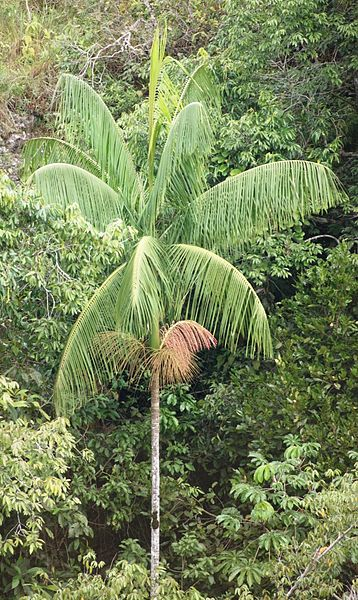
\includegraphics[width=\textwidth]{euteredulis}
  \caption{\textit{Euterpe edulis}}
  \label{fig:eeduli}
\end{subfigure}%
\begin{subfigure}[b]{.4\textwidth}
  \centering
  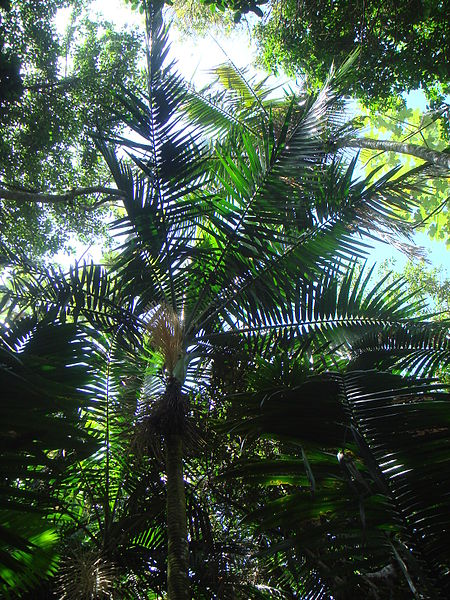
\includegraphics[width=\textwidth]{presacumimon}
  \caption{\textit{Prestoea acuminata}}
  \label{fig:pacumi}
\end{subfigure}
\begin{subfigure}[b]{.4\textwidth}
  \centering
  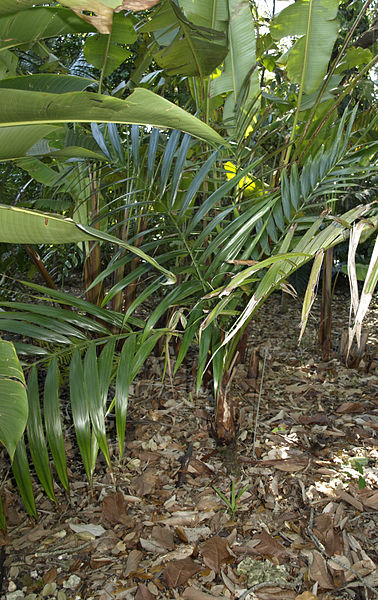
\includegraphics[width=\textwidth]{neoniwatsoni}
  \caption{\textit{Neonicholsonia watsonii}}
  \label{fig:nwatsonii}
\end{subfigure}
\begin{subfigure}[b]{.4\textwidth}
  \centering
  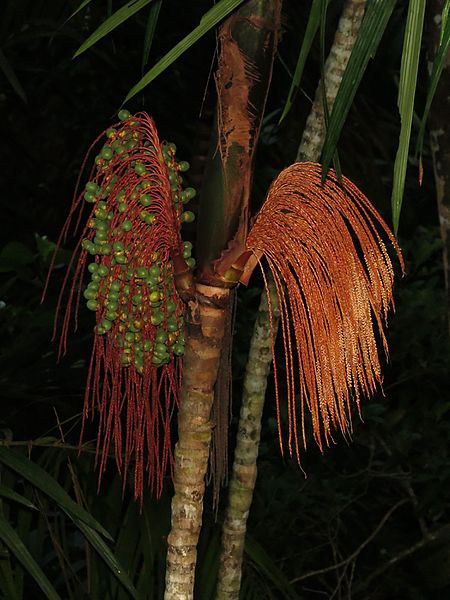
\includegraphics[width=\textwidth]{oenomapora}
  \caption{\textit{Oenocarpus mapora}}
  \label{fig:omapora}
\end{subfigure}
\caption{Genera of palm tribe Euterpeae}
\label{fig:fig}
\end{figure}
\end{comment}

\begin{figure}[!ht]
\centering
\subcaptionbox{\textit{Prestoea acuminata}\label{fig:preacumi}}
{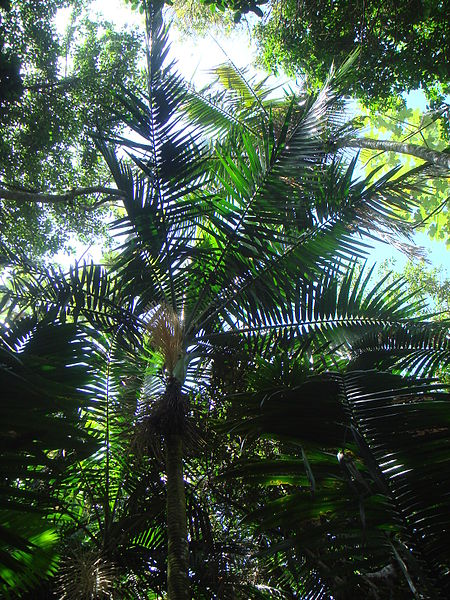
\includegraphics[width=0.4\textwidth]{presacumimon}}
\subcaptionbox{\textit{Oenocarpus mapora}\label{fig:oenomapora}}
{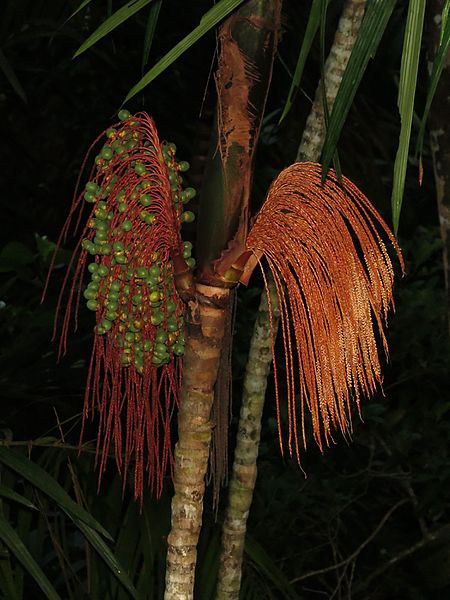
\includegraphics[width=0.4\textwidth]{oenomapora}}
\caption{Ejemplos de taxa dentro de la tribu Euterpeae}\label{animals}
\end{figure}

\lipsum[5-8]

Esto es una referencia a \textit{Prestoea acuminata} (fig.~\ref{fig:preacumi}).
Esto es una referencia a \textit{Euterpe precatoria} (fig.~\ref{fig:euterpreca}).
\begin{figure}[!hb]
\centering
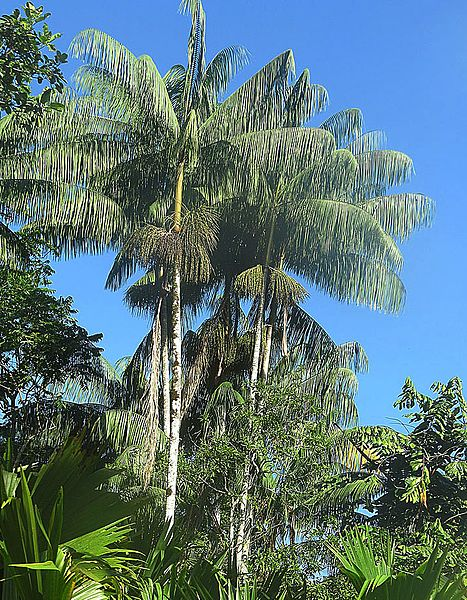
\includegraphics[width=0.5\textwidth]{eprecato}
\caption{Hábito de \textit{Euterpe precatoria}}
\label{fig:euterpreca}
\end{figure}


\chapter{Discusión}
\lipsum[1-5]
\chapter{Conclusiones}
\lipsum[1-5]
\chapter{Recomendaciones}
\lipsum[1-5]
\printbibliography[heading=bibintoc]

\etocdepthtag.toc{apendice}

\appendix


\chapter{Anexos}
\lipsum[1-2]
\section{Anexo1}
\lipsum[3-4]

\end{document}
